% !TEX root = ps4_text.tex

\documentclass[12pt]{article}

% Geometry
\usepackage[a4paper, left=3cm, right=2.5cm, top=2.5cm, bottom=3cm]{geometry}

% Font encoding
\usepackage[utf8]{inputenc} % UTF-8 encoding
\usepackage[T1]{fontenc} % Font encoding
\usepackage{times}

% Math packages
\usepackage{amsmath} % Basic math symbols and environments
\usepackage{amssymb} % Additional math symbols
\usepackage{amsfonts} % Math fonts

% Text packages
\usepackage{parskip}
\setlength{\parskip}{1em}
\usepackage{hyperref}
\hypersetup{
    colorlinks=true,
    linkcolor=blue,
}

% Pictures
\usepackage{graphicx}
\usepackage{float}

% Lists
\usepackage{enumitem}
\setlist[itemize]{itemsep = -0.5em, topsep = -0.5em}

% Bibliography
%\usepackage{cite}

% Loops:
\usepackage{pgffor}

% Extra commands:
\makeatletter
\renewcommand{\maketitle}{
  \begin{center}
    {\Huge \@title}\\[2em]
    {\large \@author \hfill \@date}\\[2em]
  \end{center}
}
\makeatother


% Title and author
\title{Econometrics II - Problem Set 4}
\author{Ricardo Semião e Castro}
\date{05/2024}


\begin{document}

\maketitle

\section*{Question 1}

\subsection*{Item 1., 2., and 4.}
In the code.


\subsection*{Item 3.}
The weak PPP says that:

$$g_{exchange} = g_{price}/g_{price*}$$

Where $g$ denotes a growth rate, and $^*$ denotes an external (to Brazil) variable. We can apply our transformation to see that:

$$100ln g_{exchange} = 100ln g_{price} - 100ln g_{price*}$$

$$Z_t = 100ln g_{price} - 100ln g_{exchange} - 100ln g_{price*}$$

Where $Z_t$ should be stationary. Then, if we order our data in Exchange -- Price -- Price*, the cointegration vector is as follows:

$$(-1 ~~ 1 ~~ -1)$$


\subsection*{Item 5. and 7.}
The plot can be seen below:

\begin{figure}[H]
    \centering
    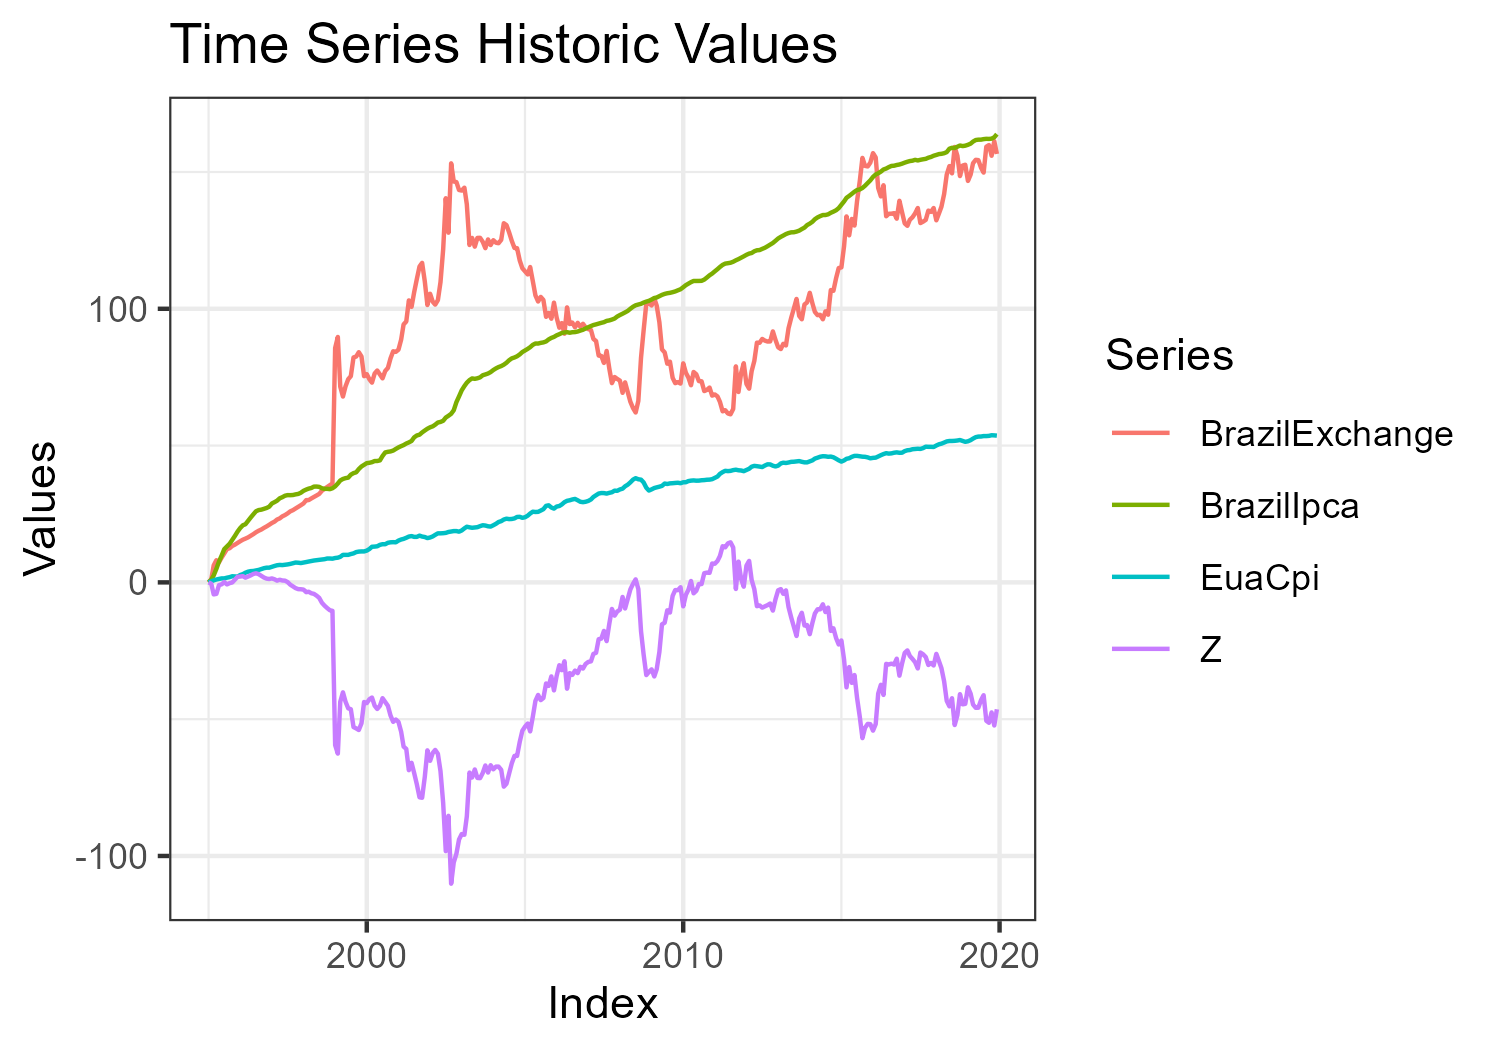
\includegraphics[width=0.9\textwidth]{figures/historic.png}
\end{figure}


\subsection*{Item 6. and 8.}
The ADF test, some considerations: the data is quarterly, so the test with 4 lags was considered; there seems to be no drift in any of the series, so only the type with trend (type 2) and the one without (type 1) were considered. The null hypothesis is a unit root in the serie. The results are as follows:


\begin{table}[!htbp] \centering 
  \caption{ADF Test - BrazilExchange} 
  \label{tb:dftest_brazilexchange} 
\begin{tabular}{@{\extracolsep{5pt}} ccc} 
\\[-1.8ex]\hline 
\hline \\[-1.8ex] 
Lag & Type 1 & Type 2 \\ 
\hline \\[-1.8ex] 
3 & 0.78
(0.87) & -1.62
(0.48) \\ 
\hline \\[-1.8ex] 
\end{tabular} 
\end{table} 


\begin{table}[!htbp] \centering 
  \caption{ADF Test - BrazilIpca} 
  \label{tb:dftest_brazilipca} 
\begin{tabular}{@{\extracolsep{5pt}} ccc} 
\\[-1.8ex]\hline 
\hline \\[-1.8ex] 
Lag & Type 1 & Type 2 \\ 
\hline \\[-1.8ex] 
3 & 3.27
(0.99) & -1.4
(0.56) \\ 
\hline \\[-1.8ex] 
\end{tabular} 
\end{table} 


\begin{table}[!htbp] \centering 
  \caption{ADF Test - EuaCpi} 
  \label{tb:dftest_euacpi} 
\begin{tabular}{@{\extracolsep{5pt}} ccc} 
\\[-1.8ex]\hline 
\hline \\[-1.8ex] 
Lag & Type 1 & Type 2 \\ 
\hline \\[-1.8ex] 
3 & 4.1
(0.99) & -1.34
(0.58) \\ 
\hline \\[-1.8ex] 
\end{tabular} 
\end{table} 


\begin{table}[!htbp] \centering 
  \caption{ADF Test - Z} 
  \label{tb:dftest_z} 
\begin{tabular}{@{\extracolsep{5pt}} ccc} 
\\[-1.8ex]\hline 
\hline \\[-1.8ex] 
Lag & Type 1 & Type 2 \\ 
\hline \\[-1.8ex] 
3 & -0.86
(0.37) & -1.8
(0.4) \\ 
\hline \\[-1.8ex] 
\end{tabular} 
\end{table} 



\subsection*{Item 9.}
We can see that the three original series have strong evidence of being I(1), as we don't reject the null hypothesis. But, the combination $Z_t$, which by the theory, should be stationary, doesn't seem so. This would mean that that exact combination is not related to a cointegration vector, and the PPP as does not hold in this context.

This can be related to the nature of the variables, there are several different ways to measure inflation, and the issue might be arising from that.



\section*{Question 2}

\subsection*{Item 1.}
I chose the order with exchange rate first, as it depends by definition on the inflation rates of the countries, thus, it should be associated with an element different than zero in the cointegration vector. The other two variables don't have a clear preference, but i choose the brazilian IPCA and then the EUA's CPI.


\subsection*{Item 2. and 5.}
The cointegration vectors were as below:


\begin{table}[!htbp] \centering 
  \caption{} 
  \label{tb:coint_vecs} 
\begin{tabular}{@{\extracolsep{5pt}} ccc} 
\\[-1.8ex]\hline 
\hline \\[-1.8ex] 
BrazilExchange & BrazilIpca & EuaCpi \\ 
\hline \\[-1.8ex] 
1 & -3.24742747968283 & 7.38509383645897 \\ 
-0.111746374798268 & 1 & -2.61391995155696 \\ 
0.0364435984264183 & -0.374855197298497 & 1 \\ 
\hline \\[-1.8ex] 
\end{tabular} 
\end{table} 



\subsection*{Item 3., 4., and 5.}
The used test was again the ADF test, with 4 lags for quarterly data. This time, there doesn't appear to be drift nor trend, so only type 1 was considered. The null is a I(1) process, but as the values for it are the estimated residuals, the critical values must be corrected.

Taking from the table B.9 from Hamilton, the values should be less than $-4.5$ to be considered I(0).


\begin{table}[!htbp] \centering 
  \caption{PO Test - BrazilExchange} 
  \label{tb:po_brazilexchange} 
\begin{tabular}{@{\extracolsep{5pt}} cc} 
\\[-1.8ex]\hline 
\hline \\[-1.8ex] 
Lag & Type 1 \\ 
\hline \\[-1.8ex] 
3 & -2.02
 \\ 
\hline \\[-1.8ex] 
\end{tabular} 
\end{table} 


\begin{table}[!htbp] \centering 
  \caption{PO Test - BrazilIpca} 
  \label{tb:po_brazilipca} 
\begin{tabular}{@{\extracolsep{5pt}} cc} 
\\[-1.8ex]\hline 
\hline \\[-1.8ex] 
Lag & Type 1 \\ 
\hline \\[-1.8ex] 
3 & -2.65
 \\ 
\hline \\[-1.8ex] 
\end{tabular} 
\end{table} 


\begin{table}[!htbp] \centering 
  \caption{PO Test - EuaCpi} 
  \label{tb:po_euacpi} 
\begin{tabular}{@{\extracolsep{5pt}} cc} 
\\[-1.8ex]\hline 
\hline \\[-1.8ex] 
Lag & Type 1 \\ 
\hline \\[-1.8ex] 
3 & -2.63
 \\ 
\hline \\[-1.8ex] 
\end{tabular} 
\end{table} 


Based on this analisys, the values are indeed less than $-4.5$, so the residuals are stationary, and the cointegration vectors are valid. Thus, with this more general approach, a combination of the three variables can be stationary.



\section*{Question 3}

\subsection*{Item 1. and 2}

In code (unfinished).



\end{document}
